\documentclass{article}
\usepackage{libertinus}
\usepackage{tikz}
\usetikzlibrary{matrix}
\newlength{\mydrawlinewidth}
\setlength{\mydrawlinewidth}{1pt}
\begin{document}
    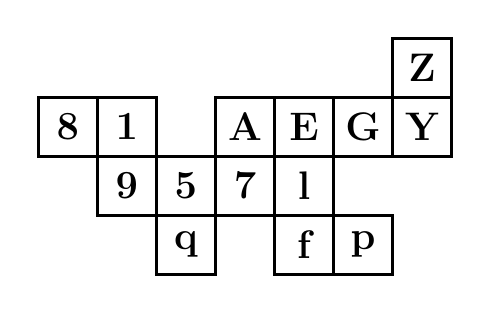
\begin{tikzpicture}
        \matrix[%
            matrix of nodes,%
            column sep=-\mydrawlinewidth,%
            row sep=-\mydrawlinewidth,
            nodes={
                rectangle,draw,
                line width=\mydrawlinewidth,
                anchor=center,
                inner sep=2pt,outer sep=0pt,
                font=\bfseries\Large,
                minimum size=.75cm,
                }
            ]
        {
          &   &   &   &   &   & Z\\ 
        8 & 1 &   & A & E & G & Y\\ 
          & 9 & 5 & 7 & l  &   &  \\ 
          &   & q &   & f & p &  \\
        };
    \end{tikzpicture}
\end{document}
